% !TeX spellcheck = en_US
\begin{frame}
\Section{Vector Spaces}
~\\~\\
\Subsection{Introduction}
~\\
Preliminary remarks:\\
\Hide{
\begin{itemize}
	\item So far, we worked with ``vectors'' in $\R^n, \F^n,..$. We introduced the notions of summation, multiplication, linear combination, span, basis,...
	\item We also summed and scaled matrices, but did not talk about a span of matrices, basis, etc...
	\item In the exercise class we considered infinite discrete signals. We could add and scale sequences in $\R^\N, \R^\Z,..$ as well and talk about linear combinations, basis, etc...
	\item Similarly, considering functions $f\colon \R \to \R$ and sets of functions (function spaces are studied in functional analysis). We could define summation and scaling. Example: Polynomials, frequencies,...
\end{itemize}
~\\~\\
We now establish a more abstract point of view and revisit notions such as vectors, linear combinations, basis, etc. once again. You will see that we have already learned all the basic ideas.
}
\end{frame}

\begin{frame}
	\begin{definition}[Group]
		Let $G$ be a set and $\ast: G \times G \to G$ a function, so that 
	\begin{itemize}
	\item[\textbf{G1}]Associativity: $\forall g_1, g_2,g_3\in G:~ g_1\ast(g_2\ast g_3)=(g_1\ast g_2)\ast g_3$
	\item[\textbf{G2}] Neutral element: $\exists e \in G~\forall g \in G: ~g \ast  e = g$
	\item[\textbf{G3}] Inverse element: $\forall g \in G ~\exists_1 g^{-1} \in G:~ g\ast g^{-1}=e$
\end{itemize} 
	 Then $(G,\ast )$ is called \textbf{group}. 
	 ~\\~\\
	 If in addition
	 	\begin{itemize}
	 	\item[\textbf{G4}] Commutativity: $\forall g_1, g_2 \in G:~ g_1 \ast  g_2 = g_2\ast g_1$,
	 \end{itemize}
 then it is called a \textbf{commutative/abelian group}.
	\end{definition}


\Hide{
	~\\
Group theory plays a crucial role in cryptography (RSA,...)
~\\
\begin{example}
	~\\
	\begin{itemize}
	\item $G = \{g\}$
	\item $(\Z,+)$
	\item $(\text{GL}(n,\R),\cdot)$; it is not commutative, take e.g., 
	$$
	\begin{pmatrix}
	0&1\\1&0
	\end{pmatrix}, 
	\begin{pmatrix}
	1&0\\0&2
	\end{pmatrix}
	$$
	In words: If both coordinates are scaled differently, then it makes a difference if we swap them before or after the scaling. 
\end{itemize}
~\\
Not a group:
\begin{itemize}
	\item $(\N,+)$, inverse element of $1$?
\end{itemize}
\end{example}

}
\end{frame}


\begin{frame}
	We now add more structure by abstracting the familiar properties of real numbers with summation (subtraction) and multiplication (division).
	\begin{definition}[Field]
		 Let $F$ be a set and $+\colon F \times F \to F$ and $\cdot:F\times F \to F$ two functions such that
		 \begin{itemize}
		 	\item[\textbf{F1}] $(F,+)$ is a commutative group (with neutral element $0$)
		 	\item[\textbf{F2}] $(F\setminus \{0\},\cdot)$ is a commutative group (with neutral element $1$)
		 	\item[\textbf{F3}] Distributivity (compatibility of $+$ and $\cdot$)
					\begin{align*}
					 a \cdot (b+c) = a\cdot b + a \cdot c\\
					 (a+b) \cdot c= a\cdot c + b \cdot c
					\end{align*} 
		 \end{itemize}
	\end{definition}
\Hide{	
	~\\~\\
	\begin{example}~\\
		\begin{itemize}
			\item $(\R,+,\cdot)$
			\item $(\Q,+,\cdot)$
			\item $(\C,+,\cdot)$
		\end{itemize}
		~\\
		Not a field:
		\begin{itemize}
			\item $(\Z,+,\cdot)$, because $(\Z\setminus \{0\},\cdot)$ is not a group (no multiplicative inverse of, e.g., $2,3,4...$)\\
			It is just a ``ring'' (with respect to multiplication it is a semigroup (no inverses) and not a group)
		\end{itemize}
	\end{example}
}
\end{frame}

\begin{frame}[c]
We now abstract the notion of vectors in $\R^n$ and their properties. 
\begin{definition}[Vector space]
Let $\F$ be a field. A set $V$ together with a function $+$ 
(sum) and a function $\cdot$ (scalar multiplication) with 
\begin{eqnarray*} \begin{array}{r@{~}lr@{~}l} 
		+: V \times V & \to V & \cdot : \F \times V & \to V \\ 
		(v,w)       & \mapsto v+ w    & (\lambda, v) & \mapsto \lambda \cdot v  
\end{array} \end{eqnarray*} 
is called \emph{\textbf{vector space (or linear space)} over $\mathbb{F}$}, if the following axioms \textbf{VR1} and \textbf{VR2} hold: 

\begin{itemize} 
	\item[\textbf{VR1}] $(V,+)$ is a commutative group with neutral element $0$.%, i.e., 
%	\begin{itemize}\normalsize
%		\item[\textbf{G1}]Associativity: $\forall v_1, v_2,v_3\in V:~ v_1+(v_2+v_3)=(v_1+v_2)+v_3$
%		\item[\textbf{G2}] Neutral element: $\forall v \in V: ~v + 0 = v$
%		\item[\textbf{G3}] Inverse element: $\forall v \in V ~\exists_1 (-v) \in V:~ v+(-v)=0$
%		\item[\textbf{G4}] Commutativity: $\forall v_1, v_2 \in V:~ v_1 + v_2 = v_2+v_1$
%	\end{itemize}
	\item[\textbf{VR2}] The scalar multiplication is compatible with 
	$(V,+)$ in the following way:  
	
	for $\lambda,\mu \in \F$, $v,w \in V$ it holds that  
	\begin{itemize} \normalsize
		\item[i)] $(\lambda + \mu)\cdot v = \lambda \cdot v + \mu \cdot v$ 
		\item[ii)] $\lambda \cdot (v+w) = \lambda \cdot v + \lambda \cdot w$ 
		\item[iii)] $\lambda \cdot (\mu \cdot v) = (\lambda \cdot \mu) \cdot v$  
		\item[iv)] $1 \cdot v = v$ 
	\end{itemize} 
\end{itemize}
\end{definition}
Remarks:
\begin{itemize}
	\item The vector space axioms allow for an abstract study and serve as an interface to the developed theory. For example, this is important for the study of linear equations, where the sought after solutions are functions (e.g., differential or integral equations). We then look for solutions in particular function spaces (typically infinite--dimensional which we approximate with finite--dimensional ones on the computer).
	\item Often one equips vector spaces with additional structure: Norm (abstract notion of length), inner product (relates to angles and orthogonality), topology (relates to limits, continuity and connectedness),...\\
	$\rightarrow$ Below we will introduce inner product spaces (a preliminary stage to so-called Hilbert Spaces)
\end{itemize}
\end{frame}


%%
\begin{frame}
\begin{example}
	\Hide{ ~\\
\begin{itemize}
    \item[(i)] $\R,~ \C,~ \R^n,~ C^n,~ \R^{m\times n}$\\
~\\
Let us verify the axioms for $\R^{m\times n}$. We have defined matrix sum $+$ and scaling $\cdot$.\\ ~\\
\textbf{(VR1)} $(\R^{m\times n}, +)$ is a commutative group:\\
...\\
~\\
\textbf{(VR2)} Recall the compatibility properties from Lemma \ref{lem:compatibility_sum_scale}:\\
Let $A,B \in \R^{m\times n}$ and $r,s \in \R $. Then 
\begin{eqnarray*} 
	\begin{array}{lr@{~}l} 
		i)  & (r+s) \cdot A =      & r\cdot A+s\cdot A  \\ 
		ii) & r\cdot (A+B) =       & r \cdot A+r \cdot B\\
		iii)& (r\cdot s) \cdot A = & r\cdot(s\cdot A)  \\ 
		iv) & 1\cdot A = A          &    \hspace*{10cm}
	\end{array}  
\end{eqnarray*}
\end{itemize}
}
\end{example}
\end{frame}

\begin{frame}
	 \Hide{\begin{itemize}
	 		\item[(ii)] Let $V := \{ \rho \mid \rho: [0,1] \rightarrow \mathbb{R}\}$ and define
	 		$$ (\lambda \cdot \rho)(x) := \lambda \cdot \rho_2(x), 
	 		\hspace{1cm} (\rho_1 +\rho_2)(x) := \rho_1 (x) +\rho_2(x)
	 		$$\\~\\
	 		Functional analysis deals with infinite dimensional vector spaces of functions and generalizes/extends results from linear algebra.\\

	 		\begin{minipage}{\textwidth}
	 			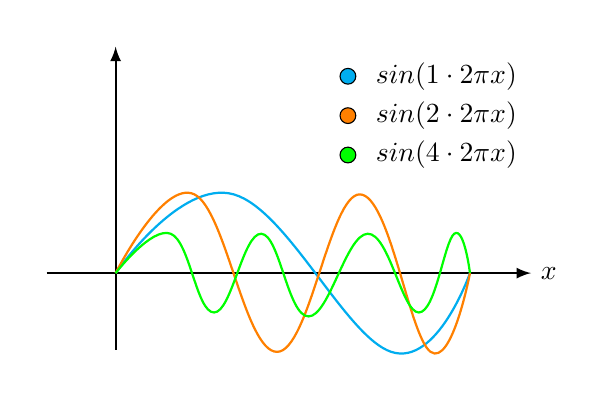
\begin{tikzpicture}
	 			\node (v2) at (-0.5,3) {};
	 			\node (v1) at (-0.5,-1.1) {};
	 			\node (v3) at (-1.5,0) {};
	 			\node (v4) at (5,0) {$x$};
	 			\draw [-latex,thick] (v1) edge (v2);
	 			\draw [-latex,thick] (v3) edge (v4);
	 			\draw [cyan,thick] plot[smooth, tension=.7] coordinates {(-0.5,0) (1,1) (3,-1) (4,0)};
	 			\draw [orange,thick] plot[smooth, tension=.7] coordinates {(-0.5,0) (0.5,1) (1.55,-1) (2.6,1) (3.5,-1) (4,0)};
	 			\draw [green,thick] plot[smooth, tension=.7] coordinates {(-0.5,0) (0.2,0.5) (0.75,-0.5) (1.35,0.5) (1.95,-0.55) (2.7,0.5) (3.35,-0.5) (3.8,0.5) (4,0)};
	 			\node at (3.7,2.5) {$sin(1\cdot2\pi x)$};
	 			\node at (3.7,2) {$sin(2\cdot 2\pi x)$};
	 			\node at (3.7,1.5) {$sin(4\cdot 2\pi x)$};
	 			\draw [fill=cyan] (2.45,2.5) ellipse (0.1 and 0.1);
	 			\draw [fill=orange] (2.45,2) ellipse (0.1 and 0.1);
	 			\draw [fill=green] (2.45,1.5) ellipse (0.1 and 0.1);
	 			\end{tikzpicture}
	 		\end{minipage}
~\\~\\
	 		\item[(iii)] Gray-scale images of size 1024 x 1024: 
	 		$$\{A\in \mathbb{R}^{1024 \times 1024} \mid a_{ij} \in [0,1]\}$$ is only a subset of a vector space, not a vector space as such. It is a convex set though.
	 \end{itemize}}
\end{frame}

 \begin{frame}
\Hide{ 
	\begin{itemize}
 	\item[(iv)] The two-dimensional sphere in $\R^3$ is defined by
 	$$S^2= \{ x\in \mathbb{R}^3 \mid \norm{x} = 1\}$$
 	for some norm $\|\cdot\|$. For the Euclidean norm it looks like this:
 	\vspace{0.5cm}
	\begin{center}
	 	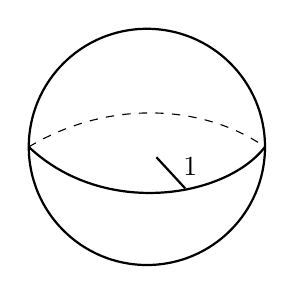
\begin{tikzpicture}
 		\draw [thick] (-1.5,1) node (v1) {} ellipse (1.5 and 1.5);
 		\draw [thick](-3,1) .. controls (-2.05,0.1) and (-0.5,0.35) .. (0,1);
 		\draw [dashed](-3,1) .. controls (-2,1.6) and (-0.8,1.55) .. (0,1);
 		\node (v2) at (-0.9,0.35) {};
 		\draw [thick] (v1) edge (v2);
 		\node at (-0.95,0.75) {1};
 		\end{tikzpicture} 
	\end{center}
 	This not a vector space (curvature prevents a simple summation of two elements), but a so-called \textbf{manifold}.
 	\item[(v)]Let $n \in \mathbb{N}$ and $P_n(\mathbb{R})$ be the set of all polynomials of degree $\leq n$ on $\mathbb{R}$, i.e., the set $P_n(\mathbb{R})$ contains all functions $p:\mathbb{R} \rightarrow \mathbb{R}$ of the form
 	\begin{align*}
 	p(x) = \sum_{k=0}^n \alpha_k x^k
 	\end{align*}
 	for some $\alpha_0, \dots,\alpha_n \in \mathbb{R}$. We define a summation and scalar multiplication:
 	\begin{align*}
 	+&\colon P_n(\mathbb{R}) \times P_n(\mathbb{R}) \to P_n(\mathbb{R}),~(p+q)(x) := p(x) + q(x),\\
 	\cdot &\colon  \mathbb{R} \times P_n(\mathbb{R}) \to P_n(\mathbb{R}),\quad\quad ~~(r\cdot p)(x) := r\cdot p(x) .
 	\end{align*}
 	Monomials $q_k: \mathbb{R} \rightarrow \mathbb{R}, \hspace{.2cm} x \mapsto x^k$ form a basis of this $(n+1)$--dimensional vector space.
 \end{itemize}
}
 \end{frame}





%%%
% LINEARLY INDEPENDENT and SPAN
%%%
\begin{frame}
\Subsection{Revisit: Linear Combination, Linear Independence, Basis}
Based on the more abstract functions $+$ and $\cdot$ we can generally define:
	\begin{definition} 
Let $V$ be a vector space over the field $\F$ and $v_1,...,v_r 
\in V$. Then, we define
\begin{itemize} 
\item[a)] \textbf{Linear combination:} 
$$
\sum^r_{j=1} \lambda_j v_j ~~\in V, ~~~~~\lambda _j \in \F
$$  
%
\item[b)] \textbf{Span (set of all linear combinations):} 
$$
\text{span}(v_1,...,v_r):= \{\sum^r_{j=1} \lambda_j v_j\colon ~~ \lambda_j \in \F\, , \; j=1,...,r\} \in V
$$ 
%As special case, we define    $\text{span} (\emptyset):= \{0\}$. 
\item[d)] The vectors $v_1,...,v_r$ are called {\bf linearly independent}, if
$$ 
\sum^r_{j=1} \lambda_j v_j = 0 \quad\Rightarrow\quad \lambda_j = 0\, , \; \forall 
j=1,...,r
$$ 
\item[e)] The vectors $v_1,...,v_r$ are called \emph{basis} of $V$, 
if
\begin{itemize}
	\item[i)] $v_1,...,v_r$ are linearly independent,
	\item[ii)] $\text{span} (v_1,...,v_r) = V$. 
\end{itemize}
\end{itemize} 
\end{definition} 
With the same proof as for $\F^n$ we can show:
\begin{corollary} \label{kor4.8} 
	For vectors $v_1,...,v_r \in V$ the following statements are equivalent: 
	\begin{itemize} 
		\item[i)] $v_1,...,v_r$ are linearly independent 
		\item[ii)] every vector $v \in \text{span} (v_1,...,v_r)$ can be uniquely linearly combined from the set 
		$\{v_1,...,v_r\}$. 
		\item[iii)] None of $v_i$ for $ i = 1,\ldots,r$ can be written as a linear combination of the other. 
	\end{itemize} 
\end{corollary}
\footnotesize
Remark: Note that these notions coincide with the ones from the linear algebra section. However, now ``vectors'' are elements from any vector space $V$ and could thus be vectors in the discrete sense, or matrices, or functions,...
\end{frame}
 
 

%\begin{frame}
%	\begin{proof} 
%	\blank  
%	\scriptsize Strategy: show (i) $\Rightarrow$ (ii) $\Rightarrow$ (iii) $\Rightarrow$ (i) \vspace{-0.2cm}
%\begin{itemize}
%    \item[a)] $(i) \Rightarrow (ii)$: $(v_1, \cdots v_r)$ linear independent, let $v \in span(v_1, \cdots ,v_r)$ be combined in two combinations: \begin{align*}
%        &r = \sum\limits_{i=1}^r \lambda_i v_i \;\text{and}\; v= \sum\limits_{i=1}^r \mu_i v_i\\
%        &\Rightarrow 0 = \sum\limits_{i=1}^r \lambda_i v_i - \sum\limits_{i=1}^r \mu_i v_i = v= \sum\limits_{i=1}^r (\lambda_i - \mu_i) v_i\\
%        &\Rightarrow \lambda_i - \mu_i =0,\;\text{since}\; v_1, \cdots,v_r \;\text{are linearly independent}\\[10pt]
%        &\Rightarrow \lambda_i = \mu_i , \;\text{i.e. linear combination is unique}
%    \end{align*}
%    \item[b)] $(ii) \Rightarrow (iii)$: \text{proof by contradiction: assume we have}\; $a_{ij}$\; \text{with}\; $v_j = \sum\limits_{i=1, i \neq j}^r v_i$\vspace{-0.2cm}
%    \begin{align*}
%        &\text{take}\; \lambda_j := -1 \Rightarrow 0 = \sum\limits_{i=1}^r \lambda_i v_i \;\text{with} \; \lambda_j = -1\\
%        &\text{but also}\; 0 = \sum\limits_{i=1}^r 0\cdot v_i\\
%        &\Rightarrow \;\text{has two different representations as linear combinations of}\; \{v_1,\cdots,v_r\}\hspace{1cm} \lightning (ii)
%    \end{align*} 
%    \item[c)] $(iii) \Rightarrow (i)$: proof by contradiction: assume $v_1, \cdots, v_r$ are linear independent $\Rightarrow \exists{\lambda_i,\cdots, \lambda_r \in \mathbb{F}}$ with $\lambda_j \neq 0$ for at least one $\lambda_j$ with:
%    \begin{align*}
%        &0= \sum\limits_{i=1}^r \lambda_i v_i = \sum\limits_{i=1,i\neq j}^r \lambda_i v_i + \lambda_j v_j\\
%        &\Rightarrow v_j = \sum\limits_{i=1,i \neq j}^r (\frac{-\lambda_i}{\lambda_j})v_i \hspace{1cm} \lightning (iii)
%    \end{align*}
%\end{itemize}
%\end{proof}
%\end{frame}





\begin{frame}
\begin{example}
	\Hide{~\\
		
		Let $V:=\mathbb{R}^{2\times 3}$, then a basis of length $6$ is given by
		~\\
		$$
		\{\begin{pmatrix}
		1 & 0 & 0 \\
		0 & 0 & 0
		\end{pmatrix}, \cdots ,\begin{pmatrix}
		0 & 0 & 0 \\
		0 & 0 & 1
		\end{pmatrix}\}$$
		~\\~\\
		Independent: $\checkmark$\\
		~\\
		Generating:
		\begin{align*}
		\begin{pmatrix}
		a_{11} & a_{12} & a_{13}\\
		a_{21} & a_{22} & a_{23}
		\end{pmatrix}
		&= a_{11} \begin{pmatrix}
		1 & 0 & 0 \\
		0 & 0 & 0
		\end{pmatrix} + a_{12} \begin{pmatrix}
		0 & 1 & 0 \\
		0 & 0 & 0
		\end{pmatrix} + a_{13} \begin{pmatrix}
		0 & 0 & 1 \\
		0 & 0 & 0
		\end{pmatrix}\\
		& + 
		a_{21} \begin{pmatrix}
		0 & 0 & 0 \\
		0 & 0 & 0
		\end{pmatrix} + a_{22} \begin{pmatrix}
		0 & 0 & 0 \\
		0 & 1 & 0
		\end{pmatrix} + a_{23} \begin{pmatrix}
		0 & 0 & 0 \\
		0 & 0 & 1
		\end{pmatrix}
\end{align*}
~\\~\\
The basis is of length $6$ and thus $\dim(V)=6 (=2\cdot 3)$.
%	
}
\end{example}
\end{frame}


%%%%
%SUBSPACES
%%%%
%%
%\begin{frame}	 
%\begin{definition}[Subspace]  
%Let $V$ be a  $\F$ vector space and $U \subset V$ a subset. $U$ 
%is called a \emph{subspace} of $V$, if \\[0.2cm]
%\begin{minipage}{1\textwidth} \centering
%	\begin{itemize}
%		\item[\textbf{UV1}]~ $U \not= \emptyset$
%		\item[\textbf{UV2}]~ $u_1,u_2 \in U \Rightarrow u_1 + u_2 \in U$
%		\item[\textbf{UV3}]~ $u \in U \, , \; \lambda \in K \Rightarrow \lambda \cdot u 
%		\in U$ 
%	\end{itemize}
%\end{minipage}
%\end{definition} 
%\vspace{-0.1cm}
%$\rightarrow$ How can subspaces look like? \textbf{UV3:} They must contain $0$ ! \\[0.2cm]
%\begin{minipage}{0.5\textwidth} \small\centering
%	-- in $\R^2$: straight lines through $0$ \\ 
%	\begin{tikzpicture}
%	\node (v4) at (0.5,-0.5) {$x_2$};
%	\node (v3) at (0.5,-3.5) {};
%	\node (v1) at (-0.5,-2.95) {};
%	\node (v2) at (4,-2.95) {$x_1$};
%	\draw [-latex] (v1) edge (v2);
%	\draw [-latex] (v3) edge (v4);
%	\draw [cyan,thick] (v3) edge (v4);
%	\draw [red,thick] (v1) edge (v2);
%	\draw [fill=red] (2,-2) ellipse (0.1 and 0.1);
%	\draw [fill=cyan] (2,-1) ellipse (0.1 and 0.1);
%	\node at (3.1,-2) {$\mathbb{R}^1 \times \{0\}$};
%	\node at (3.6,-1) {$\{0\} \times  \mathbb{R}^1  \subset \mathbb{R}^2$};
%	\end{tikzpicture}
%\end{minipage} 
%\begin{minipage}{0.5\textwidth}\small\centering
%	-- why can they not be curved lines through $0$ ?
%	\begin{tikzpicture}
%	\node (v4) at (0.5,-0.5) {$x_2$};
%	\node (v3) at (0.5,-3.5) {};
%	\node (v1) at (-1.45,-2.95) {};
%	\node (v2) at (4,-2.95) {$x_1$};
%	\draw [-latex] (v1) edge (v2);
%	\draw [-latex] (v3) edge (v4);
%	\draw [red,thick] plot[smooth, tension=.7] coordinates {(-1.35,-3.4) (-0.25,-2.4) (1.2,-3.5) (2.1,-2.3) (3,-2)};
%	\node (v5) at (-0.2,-2.45) {};
%	\node (v6) at (2.25,-2.3) {};
%	\draw [green] (v5) edge (v6);
%	\node at (-0.1,-2.15) {$v$};
%	\node at (2,-2) {$w$};
%	\draw [fill=red] (1,-2.35) ellipse (0.05 and 0.05);
%	\node (v8) at (1.1,-2) {};
%	\node (v7) at (1.55,-1.45) {};
%	\draw [-latex] (v7) edge (v8);
%	\node at (1.75,-1.15) {$\frac{1}{2}v + \frac{1}{2}w$};
%	\end{tikzpicture}
%\end{minipage}
%\textbf{Examples:} \vspace{-0.3cm}
%\begin{itemize}
%	\item[(i)] $\R \times\{0\} \subset \R^2$
%	\item[(ii)]  Krylov subspace $\mathcal{K}_d(A,b)$  is a subspace of $\R^n$ and itself a vector space
%	\item[(iii)] $C^1 ([-\pi, \pi],\R) \subset C^0([-\pi,\pi],\R) $
%\end{itemize} 
%\end{frame}


%%%%
% LINEAR FUNCTIONS
%%%%
\begin{frame}
\Subsection{Linear functions: kernel, image, matrix representation}
	\begin{definition}[Linear function] Let $V,W$ be two vector spaces over 
  $\F$. Then a function $f: V \to W$ is called an {\bf $\F$-linear 
  function}, if  
  \begin{equation*} 
f(\lambda v_1+_Vv_2) ~=~\lambda f(v_1)+_Wf(v_2) \quad \forall v_1,v_2 \in V,~\lambda \in \F . 
   \end{equation*} 
The set of all linear functions is denoted by $\text{Hom}_\F(V,W)$ (homomorphisms).\\
For $f\in\text{Hom}_\F(V,W)$ we define the \emph{\textbf{kernel}} $\kernel(f)$ and the \emph{\textbf{image}} $\im(f)$ as
\begin{align*}
\kernel(f)&:=\{v\in V\colon~ f(v)=0\} \subset V,\\[0.2cm]
\im(f)&:=\{f(v)\in W\colon~ v\in V\} \subset W.
\end{align*}
\end{definition} 
  
\Hide{  ~\\
\begin{example}~\\
\begin{itemize}
	\item[(i)] $0: V \to W,~ v \mapsto 0 \in W$\\[0.1cm]
	Check:~~~ $0(\lambda v_1+v_2)=0 = 0+0 = \lambda0(v_1)+0(v_2)~~~\forall v_1,v_2 \in V,~\lambda \in \F . $
	~\\
\item[(ii)] $\text{id}\colon V \to V, ~v \mapsto v$\\[0.1cm]
Check:~~~  $\text{id}(\lambda v_1+v_2)=\lambda v_1+v_2= \lambda \text{id}(v_1)+$id$(v_2)~~~\forall v_1,v_2 \in V,~\lambda \in \F . $
~\\
\item[(iii)] If $\{v_1,...,v_n\}$ is a basis of $V$ and $\lambda \in 
  \F^{n}$ the coordinate representation of $v\in V$, i.e., $v=\sum^n_{i=1} \lambda_i 
  v_i$. Then, the function 
$$
\pi_i:  V \to \F,~~        v \mapsto \lambda_i 
$$
is linear.
~\\
\item[(iv)] The derivative $\frac{d}{dx}$ and the integral $\int$ operators are linear functions.
\end{itemize}
\end{example}
}

%
% props of kernel, image,...
%
%\begin{frame}
%	\begin{lemma}
%		Let $f\in\text{Hom}_\F(\F^n,\F^m)$. Then
%		\begin{itemize}
%			\item[(i)] $\kernel(f) \subset \F^n$ and $\im(f)\subset \F^m$ are subspaces,
%			\item[(ii)] $\rank(A_f)=\dm(\im(f))$,
%			\item[(iii)] $\kernel(f)=\{0\}\Leftrightarrow f$ is injective.
%		\end{itemize}
%	\end{lemma}
%	\begin{proof}\small
%		\blank
%		$ker(f)$ is subspace of V, because: \\
%		i) $ker(f) \subset V$ by definition\\
%		ii) $v_1,v_2 \in ker(f) \Rightarrow f(\alpha v_1 + \beta v_2) = \alpha \underbrace{f(v_1)}_{0} + \beta \underbrace{f(v_2)}_{0} =0 \Rightarrow \alpha v_1 + \beta v_2 \in ker(f)$\\
%		iii) $ker(f) \neq \emptyset$, since $\{0\} \subset ker(f)$
%		$im(f)$ is subspace of W, because:\\
%		i) $im(f) \subset W$, by definition\\
%		ii) $w_1,w_2 \in im(f) \Rightarrow \exists v_1,v_2: w_1 = f(v_1), w_2 = f(v_2)$\\
%		$\Rightarrow \alpha w_1 + \beta w_2 = \alpha f(v_1) + \beta f(v_2) = f\underbrace{(\alpha v_1 + \beta v_2)}_{=V} \in im(f)$\\
%		iii) $im(f) \neq \emptyset$, since $\{0\} \subset im(f), f(0) = 0$\\~\\	
%		The subspace property is an obvious consequence of the linearity of $f$. $\rank(f)$ is defined via SVD of a representing matrix
%		$A=U\Sigma V^\top$. Its diagonal matrix $\Sigma$ is as square root of eigenvalues independent of the specific basis choice. If $k\in\N$ is the maximal number such that $\sigma_1,\ldots, \sigma_k\neq 0$, then the first $k$ columns of $U$ form a basis of $\im(A)$. Thus $\dim(\im(f))=\dim(\im(A))=k=\rank(A)=\rank(f)$. \\
%		Injectivity: $f(u)=f(v) \Leftrightarrow f(u-v)=0$.
%	\end{proof} 
%\end{frame}

\end{frame}


	\begin{frame}[c]
			\textbf{Matrix Representation of Linear Mappings}\\~\\
		Next we show that for finite--dimensional vector spaces $V$ and $W$, say $\dim(V)=n$ and $\dim(W)=m$, the set of all linear functions from $V$ to $W$ is equivalent to the set of all $m\times n$ matrices.
		~\\~\\
		\Hide{
			\textbf{Introductory example:} \\
			Let us consider polynomials of degree no higher than $2$, i.e., $\mcP_2(\R)$. 
			Then an example of a linear function from $\mcP_2(\R)$ ($n=3$) to $\mcP_1(\R)$ ($m=2$) is given by the derivative $f(\cdot):= \frac{d}{dx}(\cdot)$.\\
			~\\
			Examples:
			\begin{itemize}
				\item $p(x)=x+2x^2 ~~~ \simeq (0,1,2)$
				\item[] $\frac{d}{dx}p(x)  = 1+4x~~~ \simeq (1,4)$
				\item $p(x)=1+3x^2 ~~~ \simeq (1,0,3)$
				\item[] $\frac{d}{dx}p(x)  = 6x~~~ \simeq (0,6)$
			\end{itemize}
			~\\
			In terms of the coordinates, the derivative $\frac{d}{dx}$ can be represented by the matrix 
			$$
			\begin{pmatrix}
			0&1&0\\
			0&0&2
			\end{pmatrix}.
			$$
			\demo{commutative diagram}
		}
		
	\end{frame} 

\begin{frame}
\Hide{
\textbf{In general}~\\~\\
Let $V$ and $W$ be finite--dimensional vector spaces over $\F$ with $\dim(V)=n$ and $\dim(W)=m$ and bases $\{v_1,\ldots,v_n\}$ and $\{w_1,\ldots,w_m\}$, respectively.
~\\~\\
Then for all $1\leq j \leq n$ we can represent the $f(v_j) \in W$ in the basis of $W$, i.e., for some numbers $(a_{ij})_{1\leq i\leq m} \in \F^m$ we find 
$$f(v_j) = \sum_{i=1}^m a_{ij} w_i .$$
Given these fixed bases for $V$ and $W$, we define the matrix 
$$ {\cal M}_{ \{w_1,\ldots,w_m\}}^{\{v_1,\ldots,v_n\}}(f) := (a_{ij})_{1\leq i \leq m,1\leq j \leq n} \in \Fmn.$$
Since any $v \in V$ can be written as 
$$v = \sum_{j=1}^n \lambda_j v_j,$$
for some $\lambda_j \in \F$,
we find by linearity of $f$ and associativity that
\begin{equation}\label{eq:linmap-as-mat}
f(v) = f(\sum_{j=1}^n \lambda_j v_j) =  \sum_{j=1}^n \lambda_j f( v_j) =  \sum_{j=1}^n \lambda_j  \sum_{i=1}^m a_{ij} w_i =   \sum_{i=1}^m \left(\sum_{j=1}^n \lambda_j a_{ij}\right) w_i =   \sum_{i=1}^m \left({\cal M}_{ \{w_1,\ldots,w_m\}}^{\{v_1,\ldots,v_n\}}(f)\cdot \lambda \right)_i w_i.
\end{equation}
Modulo the representation in the bases we see that at the core of the evaluation $f(v)$ the matrix vector product 
$${\cal M}_{ \{w_1,\ldots,w_m\}}^{\{v_1,\ldots,v_n\}}(f)\cdot \lambda, $$
which translates the coordinates accordingly.

\demo{Draw commutative diagram.}
}
\end{frame}


\begin{frame}
	\begin{remark}~\\
		\begin{itemize}
				\item The matrix ${\cal M}_{ \{w_1,\ldots,w_m\}}^{\{v_1,\ldots,v_n\}}(f)$ is sometimes called \textit{transformation matrix} (in German: \textit{Darstellungsmatrix}).
				\item It is the matrix representation of $f$ under the given bases and it tells us how to transform the coordinates!
			\item Also, it establishes a one-to-one relation between $\text{Hom}_\F (V,W)$ and $\F^{m\times n}$, i.e., $$\text{Hom}_\F (V,W)\simeq \F^{m\times n}.$$
		\end{itemize} 
	\end{remark}
\Hide{
	\begin{example}~\\
	 \begin{itemize}
	 	\item[i)] Exercise: Let $f \in \text{Hom}_\F(\F,\F)$ and $v_1\neq 0 \neq w_1$ two real numbers, each forming a basis of $\F$.
	 	\item[ii)] Let $f \in \text{Hom}_\F(\Fn, \Fm)$ and consider the two bases $V=(v_1,\ldots,v_n)\in \text{GL}_n(\F)$, and $W=(w_1,\ldots,w_m)\in \text{GL}_m(\F)$. Note that the basis vectors are now vectors in our sense so far and we can now stack them into matrices. Also, for simplicity we write
	 	$$\mcM_W^V(f) := {\cal M}_{ \{w_1,\ldots,w_m\}}^{\{v_1,\ldots,v_n\}}(f).$$
	 	We observe
	 	$$f(v_j) = \sum_{j=1}^m a_{ij}w_j ~~\Leftrightarrow~~ (a_{ij})_i = W^{-1}f(v_j), $$
	 	so that the representing matrix of $f$ is given by
	 	$$\mcM_W^V(f) := W^{-1}(f(v_1),\ldots,f(v_n)) \in \F^{m\times n}$$
	 	and 
	 	$$f(v) = f(VV^{-1}v) =  W \mcM_W^V(f) V^{-1} v. $$
	 	\demo{ Draw commutative diagram.}
	 \end{itemize}
\end{example}
}
\end{frame}

\begin{frame}
	\Hide{	
	 \begin{itemize}
	\item[iia)] Take for example $f(v):= Av$ for some $A \in \F^{m \times n}$, so that $ f \in \text{Hom}_\F(\Fn, \Fm)$. Then 
	$$\mcM_I^I(f) = ...= A $$
	and 
	$$\mcM_W^V(f) = ... = W^{-1} A V $$
	\item[iib)] In particular, if $m=n$ (so we can choose the same basis for $V=W=\F^n$), we observe
		$$\mcM_I^I(f) = ...= A $$
	and 
	$$\mcM_V^V(f) = ... = V^{-1} A V .$$
	Observations:
	\begin{itemize}
		\item $\mcM_I^I(f)$ and $\mcM_V^V(f)$ are similar. Hence, they have the same eigenvalues.	
		\item The matrix representation depends on the chosen basis, but the somewhat deeper properties (eigenvalues,...) of the linear map as such are unchanged. 
		\item This leads to the idea of searching for a particular basis in order to get a matrix representation, which reveals the ``essence'' of the respective linear function. If the eigenvectors form a basis then they would be a good choice: In this case the matrix representation is diagonal having precisely the eigenvalues on its diagonal.
	\end{itemize}
\end{itemize}

}
\end{frame}


\begin{frame}
	\Hide{	
		\begin{itemize}
			\item[iii)] Consider 
			$$\text{Hom}_\R(\R^n,\R) = \{f\colon \R^n \to \R: f~ \text{linear}\} ~~~\text{(dual space of $\Rn$)}.$$
			Let $V=(v_1,\ldots, v_n)\in \text{GL}_n(\R)$ and $\{1\}$ be a bases for $V$ and $\R$, respectively. Then for $f\in\text{Hom}_\R(\R^n,\R)$ obviously $f(v_j) = f(v_j) \cdot 1$, so that
			$${\cal M}_{I}^{V}(f)  = {\cal M}_{ \{1\}}^{\{v_1,\ldots,v_n\}}(f) = (f(v_1),\ldots,f(v_n)) \in \R^{1 \times n} $$
			is simply a row vector.\\
			For $v = VV^{-1}v =: V\lambda \in \R^n$ we have
			$$f(v) = \sum_{j=1}^n \lambda_j f(v_j) 
			=  {\cal M}_{ \{1\}}^{\{v_1,\ldots,v_n\}}(f)\cdot \lambda 
			=  {\cal M}_{ \{1\}}^{\{v_1,\ldots,v_n\}}(f)V^{-1} \cdot v
			=  \left(\left({\cal M}_{ \{1\}}^{\{v_1,\ldots,v_n\}}(f)V^{-1}\right)^\top, v\right)_2.$$
			~\\[-0.2cm]
			\textbf{Important observations/remarks} \small
			\begin{itemize}
				\item In words: The column vector $v_f:=\left({\cal M}_{ \{1\}}^{\{v_1,\ldots,v_n\}}(f)V^{-1}\right)^\top$ represents the linear function $f$ in the standard inner product $$f(\cdot) = (v_f,\cdot)_2 .$$ This is the finite--dimensional ``light version'' of the Riesz representation theorem.
				\item If we choose the standard basis $V=I$, then this vector is simply
				$${\cal M}_{I}^{I}(f)^\top = \begin{pmatrix}f(v_1)\\\vdots\\f(v_n)\end{pmatrix} \in  \Rn. $$
				\item In the next section we consider general inner products $(\cdot,\cdot)_A$ on $\Rn$ and how this effects the representing vector $v_f$:
				$$f(\cdot) = (v^A_f,\cdot)_A = (v_f,\cdot)_2.$$
				\item When considering the derivative $DF(x)\colon \Rn \to \R$ as a linear mapping we will call the vector ${\cal M}_{I}^{I}(DF(x))^\top$ the gradient of $F$ at point $x$ (represented in the standard basis and standard inner product).
			\end{itemize}
		\end{itemize}
		
	}
\end{frame}
 



\begin{frame}
	\Subsection{Inner Product Spaces}
	We now add more structure to a vector space: We equip it with an inner product. \\~\\
	\begin{definition}
	Let $V$ be a vector space over $\F$.
\begin{itemize}
	\item  A mapping $(\cdot,\cdot)\colon V\times V \to \mathbb{F}$ is called \textbf{inner product} on $\mathbb{F}^n$ if it satisfies:
		\begin{itemize}
			\item[i)] Hermitian: $\forall x,y \in V: ~(x,y) = \overline{(y,x)}$ ,
			\item[ii)] Linear in its second argument: $\forall x,y_1,y_2 \in V, \lambda \in \mathbb{F}: ~(x,y_1+\lambda y_2) = (x,y_1)+\lambda (x,y_2)$,
			%	\item[] $\forall x,y \in \mathbb{F}^n, r \in \mathbb{F}: ~ (x,r\cdot y)=r\cdot(x,y)$ 
			\item[iii)] Positive definite: $\forall x \in V\backslash\{0\}: ~ (x,x) > 0$.
		\end{itemize}
	\item
	We call $(V,(\cdot,\cdot))$  an \textbf{\color{defgruen} Euclidean vector space} or \textbf{\color{defgruen} inner product space}.
\end{itemize}
	\end{definition}
~\\
For simplicity we now stick to $V=\R^n$. We can show the following characterization:
\begin{theorem}
	Let $(\cdot,\cdot)\colon \Rn \times \Rn \to \R$, then
	$$(\cdot,\cdot)~\text{inner product on $\Rn$}~\Leftrightarrow~\exists A \in \R^{n\times n}_{spd}~\forall x,y\in\Rn: (x,y) :=(x,y)_A:= (x,Ay)_2.$$
\end{theorem}
In words: There is a one-to-one relation between all inner products on $\Rn$ and all symmetric and positive definite matrices in $\Rnn$. The proof is constructive and reveals that the entries of $A$ are given by
$$a_{ij} := (e_i, e_j) $$
where $e_j$ denote the standard basis vectors.
\end{frame}

\begin{frame}
\Hide{	\textbf{Final note:} \\~\\
	Let us again consider $\text{Hom}_\R(\R^n,\R)$ and now a general inner product $(\cdot,\cdot)_A$ on $\Rn$ for some spd matrix $A\in\Rnn$.\\~\\
	\textbf{Question}\\
	For $f \in \text{Hom}_\R(\R^n,\R)$ we know $f\colon \Rn \to \R$ is linear. On the other hand $(v,\cdot)_A:\Rn \to \R$ is linear for a fixed vector $v \in \Rn$ and inner product $(\cdot,\cdot)_A$, i.e., $(v,\cdot)_A\in \text{Hom}_\R(\R^n,\R)$. Thus it is natural to ask whether there is a one-to-one relation between $\text{Hom}_\R(\R^n,\R)$ and $\Rn$, i.e., can we find a unique $v^A_f \in \Rn$ for $f\in \text{Hom}_\R(\R^n,\R)$ so that $f(\cdot) = (v_f^A,\cdot)_A$?
	~\\~\\
	Yes we can: 
In fact, define $v_f := v_f^I :=\left({\cal M}_{I}^{I}(f)\right)^\top$, then using the findings from above and the properties of $A$ we get
\begin{align*}
f(v) =  \left(v_f, v\right)_2 = v_f^\top v = v_f^\top (A^{-1}A) v
= v_f^\top (A^{-1})^\top A v = ( A^{-1}v_f, Av)_2
=  ( A^{-1}v_f, v)_A.
\end{align*}
In words:
\begin{itemize}
	\item Fixing to the standard inner product $A=I$, we find
	$$v_f^I = \left({\cal M}_{I}^{I}(f)\right)^\top$$
	\item Changing to a general inner product, we find 
	$$v_f^A = A^{-1}v_f^I$$
\end{itemize}}
\end{frame}

\begin{frame}
	\textbf{The important relation to Data Science/Optimization}\\~\\
\begin{itemize}
	\item 	The gradient (times $(-1)$) of a function determines a descent direction. Moving in this direction will minimize the function\\~\\
\item	The gradient is precisely the vector representing the derivative of a function.\\~\\
\item	You will learn how to accelerate the gradient method by representing it in another inner product, e.g., the one induced by the Hessian $A=H_f(x)$ (this will give you Newton type method!).
\end{itemize}
\end{frame}